\documentclass[12pt,oneside,dvipsnames, table]{book}
\usepackage[margin=1.2in]{geometry}
\usepackage[toc,page]{appendix}
\usepackage{algorithm}
\usepackage{algpseudocode} 
% \usepackage{algpseudocode}
\usepackage{graphicx}
\usepackage{amssymb}
\usepackage{natbib}
\usepackage{lipsum}
\usepackage{caption}
\usepackage{subcaption}
\usepackage{tikz}
\usepackage{amsmath}
\usepackage{placeins}
\usepackage{listings}
\usepackage{mathtools}
\usepackage{booktabs}
\usepackage{tabularx}
\usepackage{xcolor}
\usepackage{fourier-orns}
\usepackage{hyperref} \hypersetup{ colorlinks=true, linkcolor=blue, filecolor=magenta, urlcolor=cyan, pdftitle={MTP-Phase-1}, pdfpagemode=FullScreen, }


% \usepackage{dedicatoria}

%define new command for dedicatoru page
\newcommand{\dedicatory}[1]{
    \clearpage
    \thispagestyle{empty}
    \vspace*{3cm}
    \begin{center}
        \textit{\large{#1}}
    \end{center}
    \clearpage
}


\definecolor{tableheader}{RGB}{255, 204, 153}

\newcommand{\name}{Saimadhav S}
% \newcommand{\mtptitle}{Deep Learning Models for Distribution Shift-Based Style Transfer with Image Prompts}
\newcommand{\mtptitle}{Development of Digital Twin for Warehousing}


% % %USE FOR NO FIGURES.
% \usepackage{comment}

% % % Master toggles
% \newif\ifremovefloats
% \newif\ifhideimages
% \newif\ifusedraft

% % ======= SET MODE HERE =======
% \removefloatstrue      % <--- this is the line you're asking about
% \hideimagesfalse
% \usedraftfalse
% % =============================

% \ifremovefloats
%   \excludecomment{figure}
% \else
%   \ifhideimages
%     \renewcommand{\includegraphics}[2][]{\relax}
%   \fi
%   \ifusedraft
%     \usepackage[draft]{graphicx}
%   \fi
% \fi
% --------------------------------------------------------------------


\usepackage{fancyhdr}
\pagestyle{fancy}
\fancyhf{}                % clear all header and footer fields
\fancyfoot[C]{\thepage}   % page number at bottom center
\renewcommand{\headrulewidth}{0pt}  % remove top line
\renewcommand{\footrulewidth}{0pt}  % no bottom line



\begin{document}
% \fontfamily{Times New Roman}
\captionsetup[figure]{margin=1.5cm,font=small,labelfont={bf},name={Figure},labelsep=colon}
\captionsetup[table]{margin=1.5cm,font=small,labelfont={bf},name={Table},labelsep=colon}
% \setlipsumdefault{1}

\frontmatter

\begin{titlepage}


% -------------------------------------------------------------------
% You need to edit the details here
% -------------------------------------------------------------------

\begin{center}
{\LARGE M.Tech Project Dissertation}\\[0.2 cm]
\large{on}\\ 
\linespread{1.2}\huge {\bfseries \mtptitle}\\[1 cm]
\large{\textbf{Master of Technology}}\\
\large{Stage - \textrm{I} Project Report}\\[0.3cm]
\large{by}\\[0.5cm]
{\Large\textbf{\name}}\\
\large{(Roll No. 24m1532)}\\
\Large{\textbf{Supervisor:}}\\
\Large{\textbf{Prof. Jayendran Venkateswaran}}\\

\linespread{1}


\includegraphics[width=5cm]{images/iitb_logo.jpg}\\[0.5cm]

\large{Department of} \\
Industrial Engineering and Operations Research (IEOR) \\[0.3cm] 
Indian Institute of Technology, Bombay\\
\large Mumbai 400076 India
\end{center}

\end{titlepage}











% -------------------------------------------------------------------
% Declaration
% \newpage
% \begin{center}
%         \Large
%         \textbf{Acceptance Certificate}
%     \end{center}
%     \large
%   This thesis entitled \textbf{“\mtptitle”} submitted by \textbf{\name} may be accepted for being evaluated. 
  
%   \vspace{2.cm}
%   \hspace{1cm}\hfill \line(1,0){150}
  
%   \hspace{1cm}\hfill  Prof. Balamurugan Palaniappan
  
%   \vspace{-0 cm}
%   \hspace{1 cm}\hfill \textbf{Supervisor}

%   \noindent
%   Place: \textbf{Mumbai}\\
%   Date:  \today %\hfill


% \newpage
% \begin{center}
%         \large
%         \textbf{Approval Sheet}
%     \end{center}
%     \small
%   This thesis entitled \textbf{“\mtptitle”} submitted by \textbf{\name} is approved for the degree of Master of Technology.
% . 
  
%   \vspace{2.cm}
%   \hspace{1cm}\hfill \line(1,0){150}
  
%   \hspace{1cm}\hfill  Prof. Balamurugan Palaniappan and Prof Jayendran Venkateswaram
  
%   \vspace{0cm}
%   \hspace{1cm}\hfill \textbf{Supervisor}
  
%   \vspace{2.cm}
%   \hspace{1cm}\hfill \line(1,0){150}
  
%   \hspace{1cm}\hfill  Prof. 
  
%   \vspace{0cm}
%   \hspace{1cm}\hfill
%   \textbf{Internal Examiner}
  
%   \vspace{2 cm}
%   \hspace{1cm}\hfill \line(1,0){150}
  
  
%   \hspace{1cm}\hfill  Prof. 
  
%   \vspace{0cm}
%   \hspace{1cm}\hfill
%   \textbf{External Examiner} 
  
%   \vspace{2 cm}
%   \hspace{1cm}\hfill \line(1,0){150}
  
%   \hspace{1cm}\hfill  Prof. 
  
%   \vspace{0cm}
%   \hspace{1cm}\hfill
%   \textbf{Chairperson}\\
  
%   \noindent
%   Date:  \today \\
%   \noindent
%   Place: \textbf{Mumbai}
\newpage
\begin{center}
    

\section*{\Large Declaration}
\end{center}
I affirm that this written submission is a representation of my own ideas, expressed in my own words. Wherever I have used the ideas or words of others, I have appropriately cited and referenced the original sources. I confirm that I have accurately acknowledged all sources used in the creation of this report. I also affirm that I have upheld all standards of academic integrity and honesty, ensuring that no idea, data, fact, or source has been misrepresented, fabricated, or falsified in this submission. I am aware that any breach of these principles may result in disciplinary action by the Institute and could also lead to legal consequences if sources are not properly cited or permissions were not obtained when required.\\[1cm]

\noindent Name: \name\\[1mm]
\rule[1em]{25em}{0.5pt}

\noindent Signature: 
\includegraphics[height=50mm]{images/report-sign.jpg}\\[1mm]
\rule[1em]{25em}{0.5pt}

\noindent Date: \today\\[1mm]
\rule[1em]{25em}{0.5pt}




%----------acknowledgements-----------
\chapter*{\Large \center Acknowledgement}

I would like to express my sincere gratitude to my supervisor, Prof.~Jayendran Venkateswaran, for his unwavering support, insightful guidance, and constant encouragement throughout this work. Their profound expertise and vision have continually inspired me to pursue excellence and approach every challenge with clarity and determination.

I am deeply thankful to the Department of Industrial Engineering and Operations Research (IEOR), IIT~Bombay, for providing a stimulating academic environment and the resources essential for this research. 

I would also like to extend my heartfelt thanks to the FedEx~ALFA Center at IIT~Bombay for their invaluable support during this journey.

Lastly, I am ever grateful to my parents and friends for their unconditional love, patience, and encouragement, which have been my greatest source of strength and motivation throughout this endeavor.







%---------------------------------------
% Add the dedication page
\dedicatory{Dedicated to my parents and teachers (\emph{gurus})}


% -------------------------------------------------------------------
% Abstract
% % \chapter*{\Large \center Abstract}
% % Vision systems deployed in aerial, agricultural, or outdoor environments often degrade under adverse atmospheric conditions such as fog, smog, blizzards, or sandstorms. These effects induce strong distribution shifts in image statistics, reducing the reliability of vision transformers and multimodal encoders trained on clean datasets.

% % This work explores diffusion-based generative frameworks to synthetically recreate such environmental conditions, enabling vision models to adapt and generalize effectively to real-world scenes. Foundational diffusion architectures (UNET,DDPM,Conditional Diffusion) and Vision based Detection(Vit) were implemented and analyzed, followed by an evaluation of style-adaptive frameworks such as StyleShot, InstantStyle, and CSGO under extreme environmental domains.

% % Based on an existing architecure of image to image generation, an adaption was maded on InstantStyle-Plus , a diffusion framework which integrates ResNoise and IP-Adapter modules for semantic and structural consistency, and further extend it with a Contrastive Style Descriptor (CSD) Guidance Loop for perceptually aligned, distribution-shift–aware image synthesis.

% % Building upon these insights 

% % A curated dataset spanning fog, sandstorm, forest-fire, snow, smog, and underwater domains was constructed to evaluate the framework. The proposed method achieves realistic, depth-aware stylization while maintaining semantic integrity, improving robustness for agricultural, aerial, and environmental monitoring applications.
% % \chapter*{\Large \center Abstract}
% % Vision systems deployed in outdoor and aerial settings often degrade under adverse conditions such as fog, blizzard, or storm,smog, which cause significant distribution shifts in image intensity and frequency. This work explores diffusion-based generative frameworks to synthetically recreate such conditions, enabling vision models to adapt and generalize effectively to real-world environments.

% % A focused DataSet was curated having images of extreme atmospheric conditions such as SandStorm-DustStorm, ForestFire,Storm,Fog,Smog and even Deep Trences Underwater.Thee are instrumental in assessing existing ,adaptive and proposed solutions for our use case.


% % Foundational diffusion architectures, including DDPM, DDIM, and Conditional Diffusion, were studied and implemented to understand their generative behavior. Building upon these, style-adaptive frameworks such as  StyleShot, InstantStyle, and CSGO were evaluated using state of the art Vision Transformers on the extreme atmospheric images.

% % An adapted model, InstantStyle Plus, integrating ResNoise and IP-Adapter modules for semantic and structural
% % consistency, and further extend it with a Contrastive Style Descriptor (CSD) Guidance Loop for perceptually aligned, distribution-shift–aware image synthesis.


% % Finally a novel method is introduced by integrating an existing method i InstantStyle with CSD Loss, guiding the diffusion process through contrastive style supervision to achieve distribution shift–aware image synthesis. The resulting system produces realistic, style-shifted datasets that improve the robustness of vision models for agricultural, aerial, and environmental monitoring applications.

% \chapter*{\Large \centering Abstract}

% Vision systems deployed in aerial, agricultural, and outdoor environments often degrade under adverse atmospheric conditions such as fog, smog, blizzards, or sandstorms.  
% These effects cause significant distribution shifts in image statistics, reducing the reliability of vision transformers and multimodal encoders trained on clear-weather datasets.

% This work explores diffusion-based generative frameworks to synthetically recreate such environmental conditions, enabling vision models to adapt and generalize effectively to real-world scenes.  
% A focused dataset was curated containing images of extreme atmospheric domains such as fog, smog, sandstorm, forest fire, storm, and underwater to evaluate existing, adaptive, and proposed solutions under consistent conditions.

% Foundational diffusion architectures, including U–Net, DDPM, and Conditional Diffusion, were implemented to understand their generative dynamics.  
% Building on these foundations, style-adaptive frameworks such as StyleShot, CSGO, and InstantStyle were evaluated on the curated dataset using state-of-the-art vision transformers to assess their ability to reproduce physically consistent style shifts.

% An adapted model, \textbf{InstantStyle-Plus}, was developed by extending InstantStyle with ResNoise and IP-Adapter modules for semantic and structural consistency, and further enhanced through a \textbf{Contrastive Style Descriptor (CSD)} guidance loop for perceptually aligned, distribution-shift–aware image synthesis.  

% Finally, a novel diffusion system integrating \textbf{InstantStyle with CSD loss} was introduced, guiding the denoising trajectory through contrastive style supervision to achieve physically realistic, depth-aware stylization while preserving semantic fidelity.The proposed framework demonstrates superior perceptual realism and environmental consistency, producing high-quality, style-shifted datasets that enhance the robustness of vision models for agricultural, aerial, and environmental monitoring applications.

\chapter*{\Large \centering Abstract}

Vision systems deployed in aerial, agricultural, and outdoor environments often degrade under adverse atmospheric conditions such as fog, smog, blizzards, or sandstorms.  
These effects cause significant distribution shifts in image statistics, reducing the reliability of vision transformers and multimodal encoders trained on clear-weather datasets.

This work explores diffusion-based generative frameworks to synthetically recreate such environmental conditions, enabling vision models to adapt and generalize effectively to real-world scenes.  

A focused dataset was curated containing images of extreme atmospheric domains such as fog, smog, sandstorm, forest fire, storm, and underwater to evaluate existing, adaptive, and proposed solutions under consistent conditions.

Foundational diffusion architectures, including U–Net, DDPM and Conditional Diffusion were implemented to understand their generative dynamics.  
Building on these foundations, style-adaptive frameworks such as StyleShot, CSGO and InstantStyle  were evaluated on the curated dataset using state-of-the-art vision transformers  to assess their ability to reproduce physically consistent style shifts.

An existing model, \textbf{InstantStyle-Plus}, was adapted by extending InstantStyle with ResNoise  and IP-Adapter  modules for semantic and structural consistency, and further enhanced through a \textbf{Contrastive Style Descriptor (CSD)} guidance loop for perceptually aligned, distribution-shift–aware image synthesis .  

Finally, a novel diffusion system integrating \textbf{InstantStyle with CSD loss} was introduced, guiding the denoising trajectory through contrastive style supervision to achieve physically realistic, depth-aware stylization while preserving semantic fidelity.  
The proposed framework demonstrates superior perceptual realism and environmental consistency, producing high-quality, style-shifted datasets that enhance the robustness of vision models for agricultural, aerial, and environmental monitoring applications.



% -------------------------------------------------------------------
% Contents, list of figures, list of tables
% -------------------------------------------------------------------

\tableofcontents
\listoffigures
\listoftables


% -------------------------------------------------------------------
% Main sections (as required)
% -------------------------------------------------------------------

\mainmatter


\chapter{Introduction}

Operations of a warehouse are currently monitored and taken actions by a 
warehousing professional. With Digital Twin, there is scope for automation. 
The decision-making at various levels can be automated. Digital Twin for a warehouse 
paves the way forward to automate decisions at various levels including Strategic, Tactical 
and Operational levels.

\section{Problem Statement}

State of the Art in Digital Twin for Warehouse Operations Literature, stop at the Digital Model or Digital Shadow level. This work aims to develop a 
fully integrated Digital Twin for Warehouse Operations. The idea is to first characterise a model for a warehouse scenario, followed by implementing 
an Opti-State Control approach to stay in the Optimal State. The Deadheading scenario in a warehouse is taken as the reference scenario. Then the goal is to 
continually remain in the optimal state, given the disturbances encountered by the warehouse.

% =====================================================
\chapter{Literature Survey}
\label{chap:literature_survey}


This chapter builds the theoretical foundation for the work presented in this report.  

% =====================================================
\section{Warehouse Digital Twins}
\label{sec:Warehouse DT}

The first paper reviewed, authored by Ferrari et al. \cite{Ferrari2022}, has focused on the creation 
of a Digital Shadow for an Automated Storage and Retrieval System (AS/RS) in a university
logistics lab. A detailed simulation model was developed using AnyLogic, incorporating 
discrete event and agent-based modeling. Although real-time control was not achieved, the 
model was able to provide insights into system layout and performance. A Warehouse Management 
System (WMS) and a Warehouse Control System (WCS) were used to coordinate operations such as 
order generation and storage location management. The system was designed to simulate the behavior 
of physical operations closely, though without live data feedback into the physical system. 

The approach by Lugaresi et al. \cite{Lugaresi2019}, involved a small-scale manufacturing setup using LEGO components.
A closed-loop production system with four stations (S1, S2, S3, S4) and associated buffers was designed,
controlled by LEGO® MINDSTORMS® EV3® bricks programmed with Python scripts. Two product types (A and B) 
with distinct processing times, modeled using Weibull distributions, were processed, and setup times for 
switching between product types were required by stations S2, S3, and S4, with S2’s setup time increasing 
exponentially after three consecutive type A pallets. A discrete event simulator, developed in ARENA® (Sim.doe), 
was used as the digital model, synchronized with the physical LMS through data exchange files (*.txt) containing 
buffer levels, processing times, and production status. Real-time data from the LMS were collected, the digital 
model was updated, and alternative production policies were simulated to identify the optimal response to a disruption
in the RTS framework.

In the work by Zhang et al, \cite{Zhang2026} the core idea is \emph{opti-state control}. Rather than a single optimization before execution, the system is continuously monitored.
 As the warehouse is deviated from its desired performance, there is adaptive reconfiguration of plans.  For warehouse and intralogistics research, the paper's contribution is to 
 move from digital twins as a monitoring tool, toward a closed-loop control system.
% =====================================================

% =====================================================
\section*{Summary}

Research has steadily advanced toward controllable and interpretable generation.  
Transformers introduced attention mechanisms, ViTs extended them to vision, and GANs and VAEs pioneered generative modeling.  
Diffusion unified these ideas into a stable probabilistic framework, enhanced by latent conditioning, cross-attention, and adapters like ControlNet and IP-Adapter.  
Contrastive systems such as CLIP and CSD added semantic and stylistic grounding, forming the basis for the adaptive, CSD-guided diffusion explored here.

% =====================================================
\chapter{Foundational Experiments}
\label{chap:foundational_experiments}

This chapter presents some foundational experiments conducted to get used to the sensing technologies needed as part of the Digital Twin.
% =====================================================
\section{RFID Experiments}
\label{sec:RFID_experiments}

A contactless technology called RFID (Radio Frequency Identification) is utilized for data collection and automatic identification. It eliminates the need for physical contact by using radio waves to transport data between an RFID tag and a reader. RFID tags and RFID readers are the two fundamental parts of an RFID system. A tiny electronic device called an RFID tag is affixed to the item you wish to track or identify. The tag is made up of an antenna that connects to the reader and a microchip that saves data. Active and passive RFID tags are two different categories.

Based on the MFRC522 chip created by NXP Semiconductors, the RC522 RFID module is a popular and inexpensive RFID reader/writer module. The standard frequency for RFID communication, 13.56 MHz, is where it operates.

This module supports several communication protocols, such as SPI (Serial Peripheral Interface), I2C (Inter-Integrated Circuit), and UART (Universal Asynchronous Receiver-Transmitter), and is appropriate for short-distance communication, usually within a 5 cm range.

The majority of RC522 modules include:

  a)  A 1K RFID card from MIFARE Classic
  b)  A key fob or tag

\begin{figure}[!h]
    \centering
    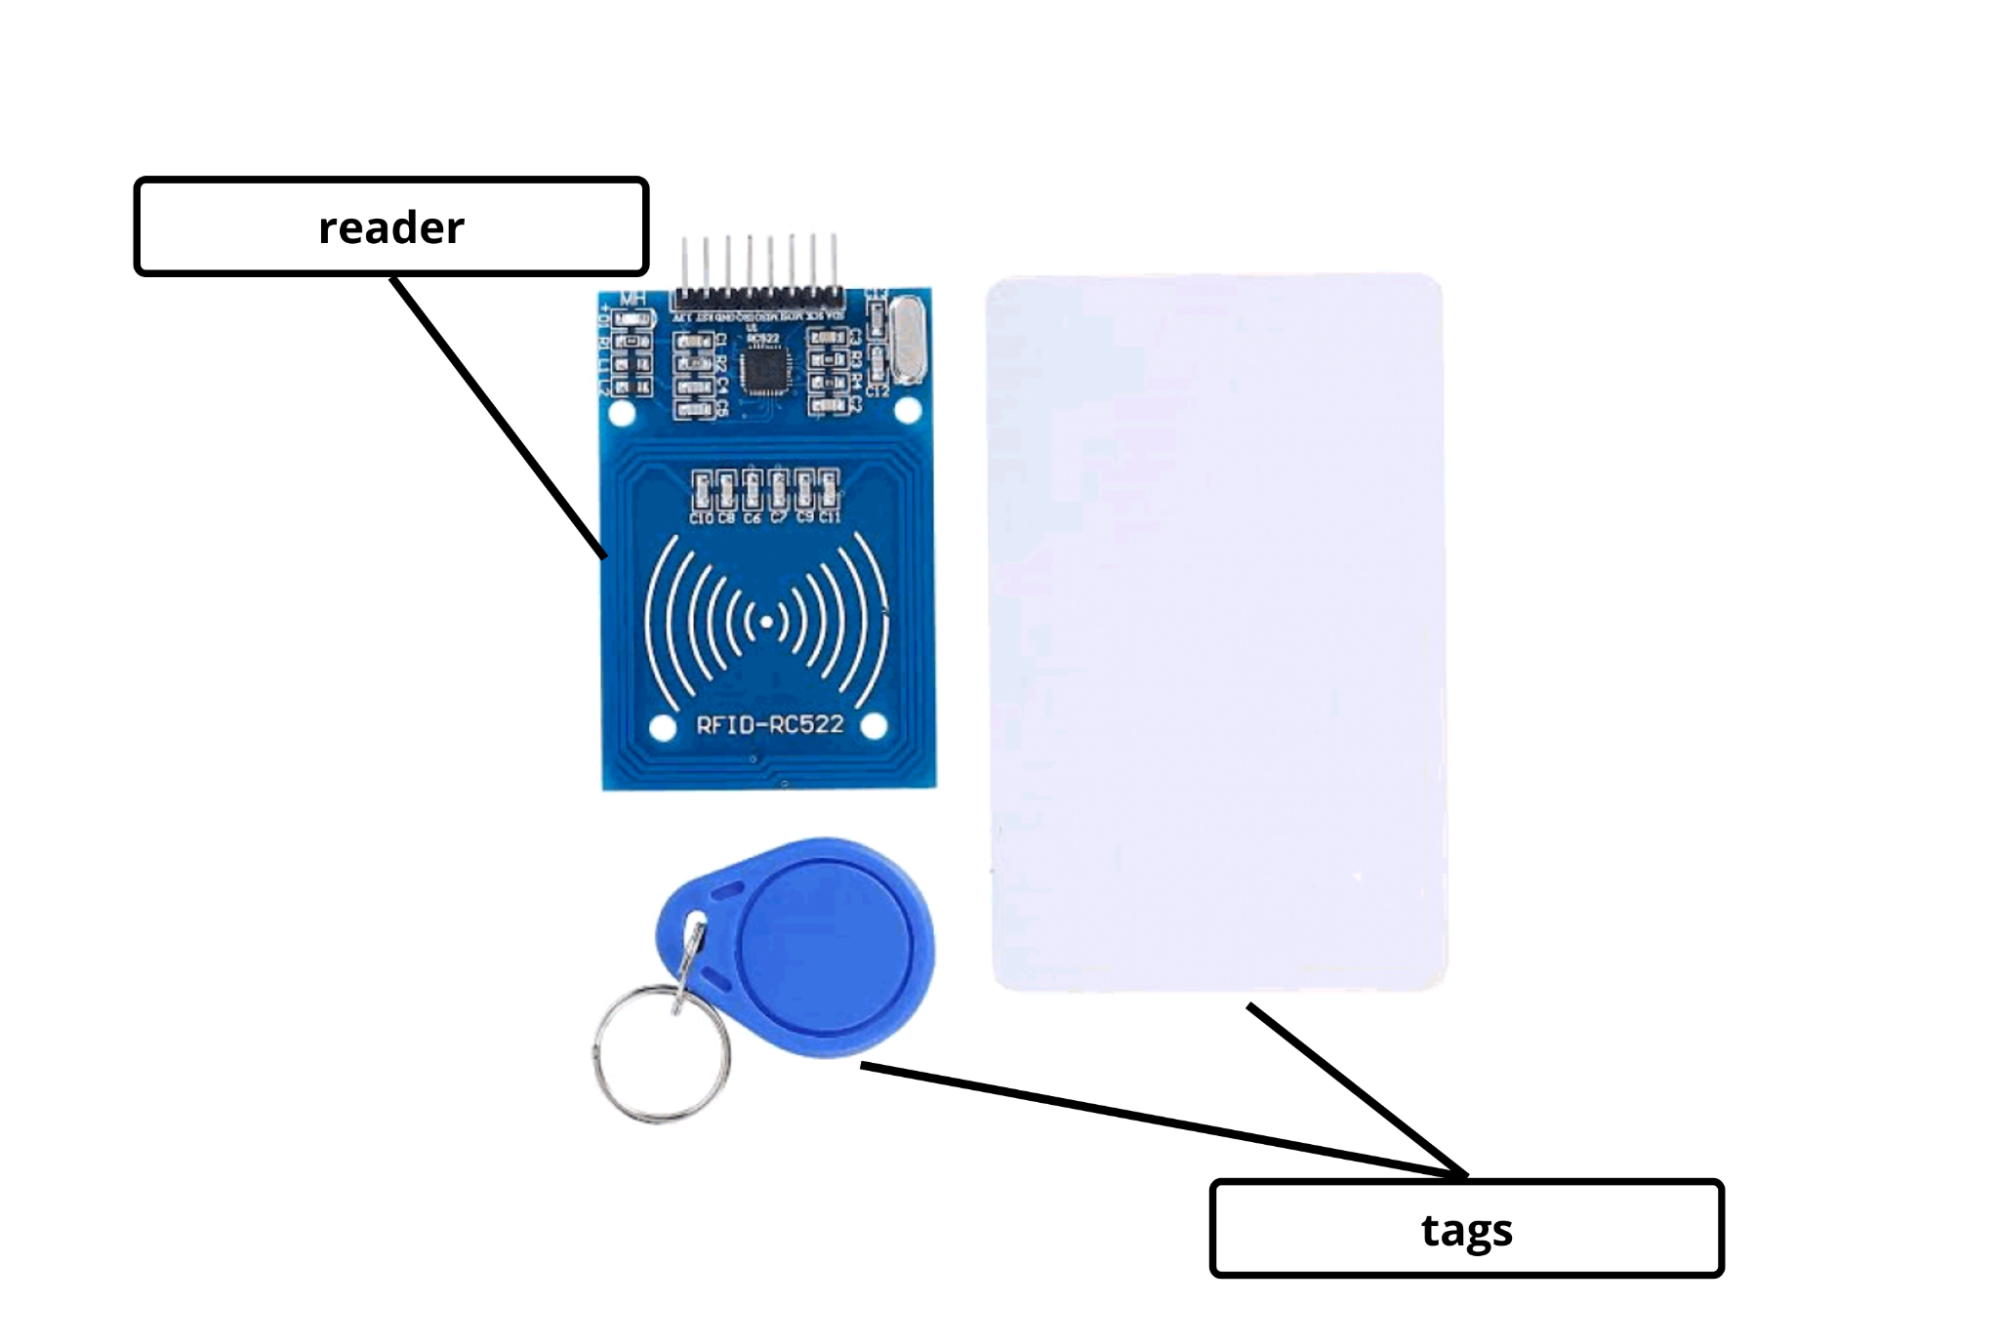
\includegraphics[width=0.65\linewidth]{images/RFID.png}
    \caption{RFID tag and reader}
    \label{fig:RFID}
\end{figure}

% =====================================================
\section{PIR sensor experiments}
\label{sec:PIR_experiment}

An electronic sensor that detects infrared (IR) light emitted by objects within its field of vision is called a passive infrared sensor (PIR sensor). PIR-based motion detectors are the most common application for them. PIR sensors are frequently utilized in automated lighting and security alarm systems. 
\begin{figure}[!h]
    \centering
    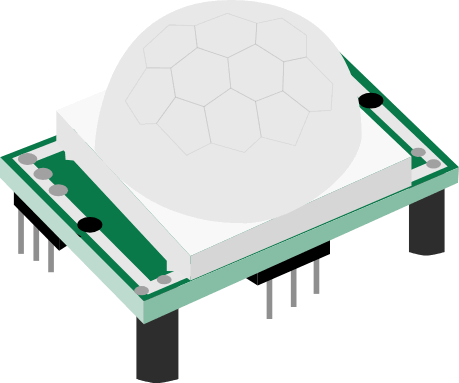
\includegraphics[width=0.55\linewidth]{images/PIR.png}
    \caption{}
    \label{fig:PIR sensor}
\end{figure}

% =====================================================
\section{Ultrasonic Sensor Experiments}
\label{sec:ultrasonic_experiments}

The ultrasonic sensor uses sound waves and the echo principle to calculate distance from obstacles. 
Distance Travelled = \frac{Speed of Sound \multiply Time Travlled}{2}
HCSR04 is the code for an ultrasonic sensor module avaialable in the market. It has a range from 2cm to 400cm. The ranging accuracy is 3mm. The sensor module has four pins: VCC, GND, TRIG and
ECHO.
\begin{figure}[!h]
    \centering
    \includegraphics[width=0.65\linewidth]{images/hcsr04.jpg}
    \caption{Ultrasonic sensor module}
    \label{fig:ddpm_samples}
\end{figure}

% =====================================================
\section{Summary of Foundational Experiments}
\label{sec:foundational_summary}

Through the above experiments, an idea of different Physical to Virtual (P2V) experiments was evaluated.

% =====================================================
\chapter{Characterisation of a model}
\label{chap:model_characterisation}

\section{Deadheading problem and the Single Cycle protocol}
\label{sec:existing_summary}

The material handling device proceeding or returning empty while attending to an order is the deadheading problem. By default or following the single cycle protocol,
when travelling to pick the item, the forklift is empty. Also, when travelling back after storing an item, the forklift is empty.

\begin{figure}[!h]
    \centering
    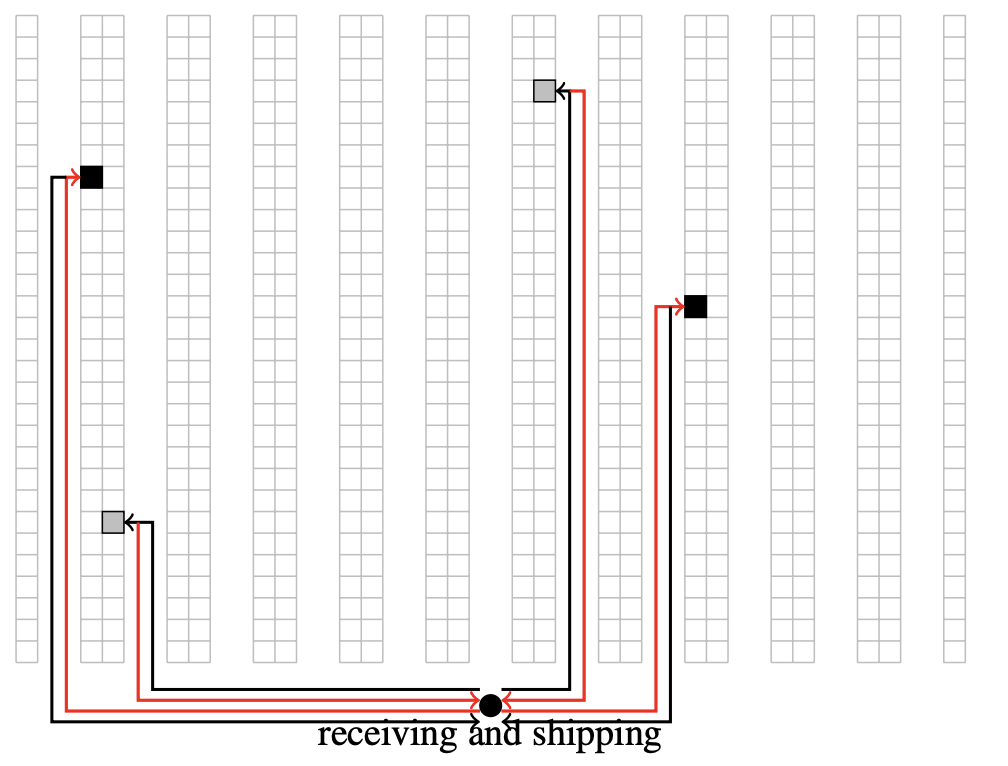
\includegraphics[width=0.65\linewidth]{images/Single_Cycle.png}
    \caption{Single Cycle Protocol}
    \label{fig:single_cycle}
\end{figure}

\section{Dual Cycle Protocol}

Enter, the dual cycle protocol. In the dual cycle protocol, a picking operation is paired with a putting (stowing) operation. This way while returning after the stow operation,
the picker proceeds to the pick operation, thereby never going empty handed.

\begin{figure}[!h]
    \centering
    \includegraphics[width=0.65\linewidth]{images/Dual_Cycle.png}
    \caption{Dual Cycle Protocol}
    \label{fig:dual_cycle}
\end{figure}

The Dual cycle protocol relies on the following optimization model: 

\begin{itemize}
    \item M is set of locations covered by store operations.
    \item N is set of locations covered by picking operations.
    \item $i \in M \text{ and } j \in N$
    \item $d_{ij}$: distance between locations $i$ and $j$
    \item $x_{ij}$: 1 if store operation at $i$ is succeeded by
    pick operation from $j$, 0 otherwise

    \begin{align*}
    \min \quad & \sum_{i,j} d_{ij}x_{ij} \\[0.2cm]
    \text{s.t.} \quad
    & \sum_i x_{ij} = 1 \qquad \forall j \\[0.1cm]
    & \sum_j x_{ij} = 1 \qquad \forall i \\[0.1cm]
    & x_{ij} \in \{0,1\} \qquad \forall i,j
    \end{align*}  
    
\end{itemize}

\paragraph{Summary}

% =====================================================
% \section{Summary}
% \label{sec:existing_summary}

% StyleShot produced aesthetic but non-physical results, CSGO provided structured disentanglement but lacked volumetric realism, and InstantStyle achieved balanced, physically grounded stylization.  
% The tuned-soft InstantStyle run proved most effective, motivating further extensions such as \textbf{InstantStyle-Plus} and \textbf{CSD-Guided Diffusion} for controlled, environment-aware adaptation.

% =====================================================
\chapter{Comparative Analysis}
\label{chap:comparison}

This chapter summarizes the comparative results across all evaluated models — StyleShot~\cite{gao2024styleshot}, CSGO~\cite{xing2024csgocomp}, InstantStyle~\cite{wang2024instantstyle}, the adapted InstantStyle-Plus~\cite{wang2024instantstyleplus}, and the proposed InstantStyle~\cite{wang2024instantstyle} + CSD~\cite{somepalli2024csd} Guidance — using both qualitative and quantitative indicators.  
The goal was not to maximize classification accuracy but to assess the \textbf{extent and realism of distribution-shift generation} under adverse environmental styles.

% =====================================================
\section{Qualitative Comparison}
\label{sec:qualitative_comparison}

Representative outputs from the curated dataset are shown in Figure~\ref{fig:qualitative_grid}.  
Across five reference prompts (\textit{tractor plowing field}, \textit{cornfield horizon}, \textit{sheep herd}, \textit{greenhouse}, and \textit{flooded crop area}), the progressive improvement in visual realism and depth consistency is clearly visible.

\begin{figure}[p]
    \centering
    \includegraphics[width=1.2\textwidth, height=0.9\textheight, keepaspectratio]{images/final_all_grid.png}
    \caption{Qualitative comparison (five representative samples) across StyleShot, CSGO, InstantStyle, InstantStyle-Plus, and Proposed model.  
    The proposed method achieves realistic environmental veiling and depth-consistent haze while preserving semantic integrity.}
    \label{fig:qualitative_grid}
\end{figure}

\noindent
\textbf{Observations:}
\begin{itemize}
    \item \textbf{StyleShot~\cite{gao2024styleshot}:} Produced overly artistic and painterly generations. While visually appealing, it performed poorly at style transfer, merely recoloring the scene without volumetric haze or realistic scattering. The model lacks depth-aware modulation, making its outputs aesthetically strong but physically implausible.
    \item \textbf{CSGO~\cite{xing2024csgocomp}:} Improved overall tonal blending but still lacked volumetric realism. Edges remained unnaturally sharp, and atmospheric style appeared as global filters rather than media that wrap around objects.
    \item \textbf{InstantStyle~\cite{wang2024instantstyle}:} Delivered the most balanced realism among existing systems, achieving physically faithful haze and turbidity while preserving prompt semantics and stable color consistency.
    \item \textbf{InstantStyle-Plus~\cite{wang2024instantstyleplus}:} Enhanced spatial and semantic stability through ControlNet~\cite{zhang2023controlnet} integration, creating smoother volumetric cues and reducing chromatic drift, though sometimes slightly softening contrast.
    \item \textbf{Proposed (InstantStyle~\cite{wang2024instantstyle} + CSD~\cite{somepalli2024csd} Guidance):} Combined all strengths—strong volumetric realism, perceptually coherent tone alignment, and stable structure—with minimal added computation.
\end{itemize}

% =====================================================
\section{Accuracy Behavior Under Distribution Shift}
\label{sec:accuracy_discussion}

To measure the perceptual domain shift caused by style generation, a Vision Transformer~\cite{dosovitskiy2020vit} classifier (ViT-B/16 trained on clear-weather images) was evaluated on the stylized outputs.  
A lower classification accuracy implies that the generated images are sufficiently distinct from the source domain—indicating a stronger, more realistic distribution shift.

\begin{table}[!h]
\centering
\caption{Classification accuracy (\%) of a ViT-B/16 model on stylized images.  
Lower accuracy implies stronger and more realistic domain shift, provided visual quality remains high.}
\begin{tabular}{|l|c|}
\hline
\textbf{Model} & \textbf{ViT Accuracy (↓)} \\ \hline
InstantStyle & 62.7 \\ 
InstantStyle-Plus & 50.9 \\ 
StyleShot & 49.0 \\ 
CSGO & 47.8 \\ 
\textbf{Proposed (InstantStyle + CSD)} & \textbf{30.3} \\ \hline
\end{tabular}
\label{tab:accuracy}
\end{table}

\noindent
The results align with qualitative observations.  
\textbf{InstantStyle} achieves the best balance of realism and prompt consistency, while \textbf{InstantStyle-Plus} and the \textbf{Proposed CSD-guided} method induce a significantly stronger and more physically meaningful domain shift, reducing ViT accuracy by nearly half.  
In contrast, \textbf{StyleShot} achieves a similar drop in accuracy but due to over-artistic distortion, not realistic environmental transfer—its outputs deviate semantically and physically from real-world phenomena.  
Thus, the \textbf{Proposed (InstantStyle + CSD)} model produces the most convincing style shift while maintaining photorealism.

% =====================================================
\section{Parameter Efficiency}
\label{sec:parameter_efficiency}

A model’s practicality depends not only on realism but also on computational footprint.  
Table~\ref{tab:param_compare} summarizes parameter statistics for each framework
\begin{table}[!h]
\centering
\caption{Parameter comparison across evaluated frameworks.}
\begin{tabular}{|l|c|c|}
\hline
\textbf{Model} & \textbf{Total Params (Billion)} & \textbf{Trainable (Million)} \\ \hline
StyleShot & 2.1–2.2 & 435–585 \\ 
CSGO & 6.6–6.7 & 650–760 \\ 
InstantStyle & 6.0 & 22 \\ 
InstantStyle-Plus & 7.2–7.5 &  600–700 \\ 
\textbf{Proposed (CSD)} & 6.6–6.7 & \textbf{22} \\ \hline
\end{tabular}
\label{tab:param_compare}
\end{table}

\noindent
Despite integrating perceptual feedback, the proposed method retains nearly the same parameter count as InstantStyle, confirming that \textbf{quality improvements stem from perceptual correction, not additional learnable modules}.  
This efficiency makes it particularly suitable for real-time or low-resource generative applications.

% =====================================================
\section{Insights}
\label{sec:discussion_overall}

From both qualitative and quantitative perspectives, the models reveal clear trade-offs:
\begin{itemize}
    \item \textbf{StyleShot~\cite{gao2024styleshot}:} Generates artistic, stylized outputs but performs poorly in physical style realism. The style overlay lacks volumetric cues, producing attractive but unrealistic results.
    \item \textbf{CSGO~\cite{xing2024csgocomp}:} Provides explicit modularity and stable fusion but requires content-based supervision to achieve realism; without it, results remain shallow.
    \item \textbf{InstantStyle~\cite{wang2024instantstyle}:} Demonstrates physically accurate scattering and atmospheric realism with excellent prompt alignment—strong generation and moderate style shift.
    \item \textbf{InstantStyle-Plus~\cite{wang2024instantstyleplus}:} Enhances structure preservation and environmental stability through ControlNet~\cite{zhang2023controlnet} conditioning, producing realistic depth-aware cues.
    \item \textbf{Proposed (InstantStyle~\cite{wang2024instantstyle} + CSD~\cite{somepalli2024csd} Guidance):} Introduces perceptual supervision that strengthens volumetric realism and style coherence while keeping parameters low, achieving the most balanced performance overall.
\end{itemize}

Overall, while lower classification accuracy corresponds to a stronger domain shift, true success lies in combining perceptual quality and physical realism.  
The proposed method satisfies both — generating style-shifted scenes that visually resemble natural atmospheric variations while remaining semantically faithful to the input prompt.

% =====================================================
\section{Summary}
\label{sec:comparison_summary}

The comparative analysis confirms that the \textbf{InstantStyle~\cite{wang2024instantstyle} + CSD~\cite{somepalli2024csd} Guidance} framework achieves the most realistic and perceptually stable environmental stylization.  
It generates distribution-shifted domains that challenge vision classifiers without sacrificing photorealism or structural integrity, outperforming all baselines in both realism and efficiency.

% =====================================================
\chapter{Conclusion and Future Work}
\label{chap:conclusion_future}

\section{Conclusion}
This study explored the evolution of diffusion-based style transfer frameworks, beginning from foundational experiments on architectures like Vision Transformers~\cite{dosovitskiy2020vit}, U–Nets~\cite{ronneberger2015unet}, and DDPMs~\cite{ho2020ddpm}, and gradually advancing toward adaptive and perceptually guided diffusion systems. The focus was to understand how these models respond to distribution shifts caused by environmental styles such as fog, haze, snow, sandstorms, and underwater scattering.
For comparitive Analysis extreme shifts were considered and through this exploration, it was observed that early frameworks like StyleShot~\cite{gao2024styleshot} and CSGO~\cite{xing2024csgocomp}, though capable of stylization, lacked volumetric realism and semantic consistency. InstantStyle~\cite{wang2024instantstyle} emerged as a more stable and physically coherent framework, offering controllable style injection through its IP-Adapter~\cite{chen2023ipadapter} mechanism. Building upon this, the adapted InstantStyle-Plus~\cite{wang2024instantstyleplus} added spatial consistency using ControlNet~\cite{zhang2023controlnet}, while the proposed InstantStyle with CSD~\cite{somepalli2024csd} Guidance integrated perceptual feedback directly into the diffusion process. This final model demonstrated the best balance between realism, controllability, and computational efficiency, producing physically consistent, depth-aware, and semantically aligned outputs. The results highlight that realistic domain adaptation through diffusion models is best achieved not by increasing complexity, but by combining adaptive structure with perceptual understanding.

\section{Future Work}
Future work can extend this research toward more physics-aware and adaptive generative pipelines. Integrating explicit depth or scattering priors into diffusion sampling could improve the realism of environmental media like fog and haze. Developing dynamic guidance schedules that adjust style strength automatically across scenes may further enhance generalization. Testing on large-scale classification and detection tasks will confirm whether these synthetic shifts enhance real-world robustness.






% appendix
% \appendix
% \input{sections/3_Key Concepts in Text Analytics.tex}
% \input{sections/2_Neural Networks and Deep Learning}
% \input{sections/6_Experimentation with DL algorithms.tex}
% \input{sections/Transformers.tex}
% \input{sections/sentence classification.tex}
% \input{sections/Named Entity Recognition.tex}

% Bibliography
\addcontentsline{toc}{chapter}{Bibliography}
\nocite{*}
\bibliography{references.bib}
\bibliographystyle{plain}

\begin{center}
----- \floweroneleft\floweroneright -----
\end{center}
\end{document}